%%%%%%%%%%%%%%%%%%%%%%%%%%%%%%%%%%%%%%%%%%%%%%%%%%%%%%%%%%%%%%%%%%%%%%%%
\chapter{Investigated Methods}\label{chap:methods}
%%%%%%%%%%%%%%%%%%%%%%%%%%%%%%%%%%%%%%%%%%%%%%%%%%%%%%%%%%%%%%%%%%%%%%%%


\noindent As seen in \ref{sec:state-of-the-art}, there are several approaches to skin detection, and it can be confusing to make a choice.
All the different categories of methods are characterized by certain strength and weaknesses, therefore the choice to implement an approach should be made carefully.\\
\textbf{Rule-based} techniques represent a simple method to rapidly separate objects from their surroundings, don't require training, and generally are easy to implement.
However, color is the only feature they consider, and therefore the classification on backgrounds with skin-like colors, such as wood or clay, could be difficult.\\
\textbf{Machine learning} approaches are suitable when there is training data available.
There are several techniques with different features in this category.
Some uses only pixels color has the main drive for classification, while others manage to consider multiple features.\\
\textbf{Hybrid} methods are suitable when a single classification technique does not produce the desired results.

The chosen methods belong to the following categories: thresholding, traditional machine learning, deep learning.\\
Thresholding has been chosen because of the simplicity of the approach, which may demonstrate how powerful simple rules can be.\\
Machine learning and deep learning have been chosen for a comparison of their classification ability: it might be interesting to see how CNNs can learn about semantics from images~\cite{dharmaretnam2018emergence} and the comparison with respect to the traditional models.\\


\FloatBarrier
%%%%%%%%%%%%%%%%%%%%%%%%%%%%%%%%%%%%%%%%%%%%%%%%%%%%%%%%%%%%%%%%%%%%%%%%
\section{Thresholding}
%%%%%%%%%%%%%%%%%%%%%%%%%%%%%%%%%%%%%%%%%%%%%%%%%%%%%%%%%%%%%%%%%%%%%%%%

Thresholding methods are based on the idea that human skin can be grouped in clusters within a color space.
Therefore, the main process is to define the boundaries of the clusters.
Color images are segmented by designating separate thresholds for each color component, as seen in \autoref{fig:thresh-cube}.
The pixels falling within the range of these thresholds are classified as skin pixels.

There are static and dynamic thresholding methods.
\textbf{Static thresholding} consists of simple fixed rules to define the cluster boundaries.
In \textbf{Dynamic thresholding} the rules defining the boundaries depend on some variables.

\begin{figure}[h]
    \centering
    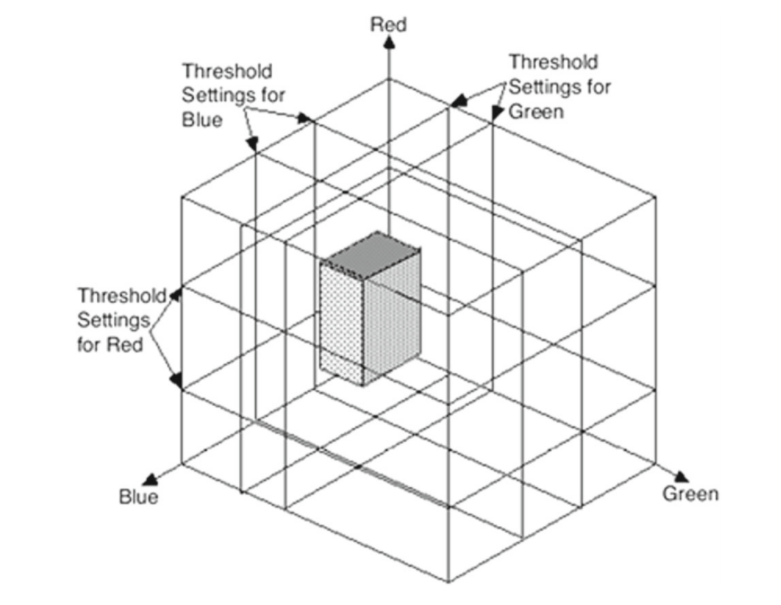
\includegraphics[width=0.7\linewidth]{images/approaches/thresholding/thresh_cube.png}
    \caption{Separate threshold settings for each color component.
    The shaded area is the Boolean AND of the three threshold settings. Adapted from John C. Russ 2007~\cite{zbMATH05833717}}
    \label{fig:thresh-cube}
\end{figure}

In literature, there isn't an agreement on the best color space to use. Nonetheless, to select the most suitable color space, its features should be taken into account.
For example, RGB describes a high correlation between color channels. An interesting technique to increase the detector accuracy is to combine channels of different color spaces~\cite{bin2007rgb}.
Several color spaces have been tested over the years: RGB~\cite{kovac2003human, cheddad2009skin, chen2012statistical}, RGB-H-CbCr~\cite{bin2007rgb}, HSV~\cite{garcia1999face, baskan2002projection, do2007skin}, YUV~\cite{yao2001face, vadakkepat2008multimodal}, YCbCr~\cite{garcia1999face, vadakkepat2008multimodal,  brancati2017human}.
Despite their simplicity, thresholding methods are relevant because of their low computational cost.
Their efficiency makes hardware implementations suitable, for example on Field Programmable Gate Array (FPGA)~\cite{chen2012statistical}.\\
An example of threshold rules in the RGB color space is presented below (taken from Kovac \textit{et al}. 2003~\cite{kovac2003human}):

\begin{minipage}{\linewidth}
\begin{verbatim}
    # The skin colour at uniform daylight illumination
    R > 95 AND G > 40 AND B > 20 AND
    max{R, G, B} - min{R, G, B} > 15 AND
    |R - G| > 15 AND R>G AND R>B
    
    OR
    
    # The skin colour under flashlight or (light) daylight
    # lateral illumination
    R > 220 AND G > 210 AND B > 170 AND
    |R - G| <= 15 AND R>B AND G>B
\end{verbatim}
\end{minipage}


\FloatBarrier
%%%%%%%%%%%%%%%%%%%%%%%%%%%%%%%%%%%%%%%%%%%%%%%%%%%%%%%%%%%%%%%%%%%%%%%%
\subsection{Implementation}\label{sec:impl-thresh}
%%%%%%%%%%%%%%%%%%%%%%%%%%%%%%%%%%%%%%%%%%%%%%%%%%%%%%%%%%%%%%%%%%%%%%%%

The chosen implementation\footnote{Source code available at \url{https://github.com/nadiabrancati/skin\_detection/}} is a dynamic thresholding approach~\cite{brancati2017human} published in 2017.
An overview of the algorithm is presented below:

\begin{enumerate}[Step 1:]
\item RGB to YCbCr conversion
\item Computation of $Cr_{max}$ and $Cb_{min}$
\item Pixel-wise computation of correlation rules parameters
\item Pixel-wise correlation rules check
\end{enumerate}

The method works in the YCbCr color space, so the first thing it does is the conversion of an RGB input image by using the ITU-R BT.601-5 conversion~\cite{bt2011studio}.
The skin pixels clusters assume a trapezoidal shape in the YCb and YCr color subspaces, as seen in \autoref{fig:trapeze-illuminations}.
Moreover, the shape and size of the trapezium vary according to many factors, such as the illumination conditions. 

In high illumination conditions, the base of the trapezium results larger.
Besides, the chrominance components of a skin pixel P with coordinates ($P_Y$, $P_{Cb}$, $P_{Cr}$) in the YCbCr space exhibit the following behavior: the further is the ($P_Y$, $P_{Cr}$) point from the longer base of the trapezium in the YCr subspace, the further is the ($P_Y$, $P_{Cb}$) point from the longer base of the trapezium in the YCb subspace, and vice versa.

\begin{figure}[h]
    \centering
    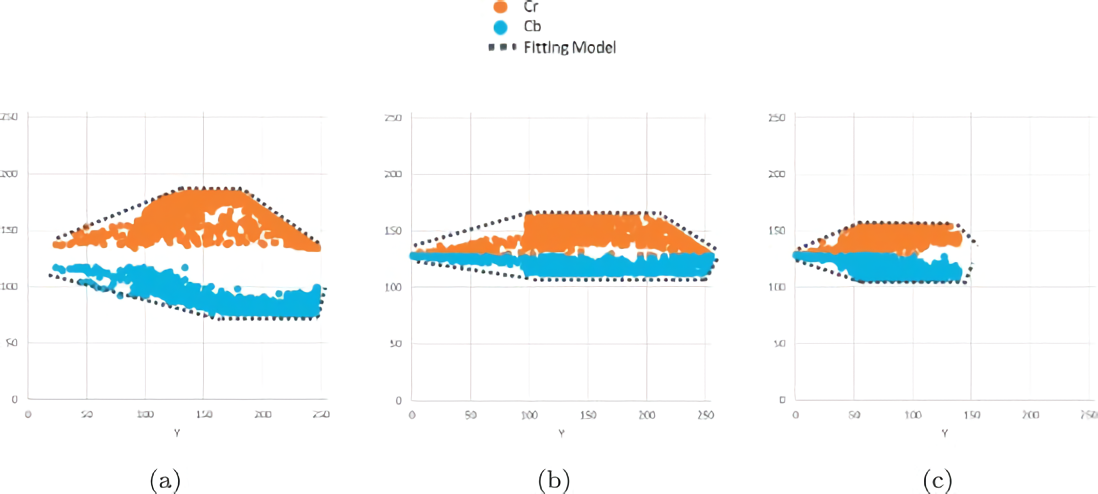
\includegraphics[width=0.9\linewidth]{images/approaches/thresholding/trapezia_illuminations.png}
    \caption{Fitting model for the YCb and YCr subspaces, in different conditions of illumination: (a) indoors with artificial light (b) outdoors with sunlight and (c) with low lighting.
    Adapted from Brancati \textit{et al.} 2017~\cite{brancati2017human}.}
    \label{fig:trapeze-illuminations}
\end{figure}

The aforementioned observations are the base of the method: it tries to define image-specific trapeziums in the YCb and YCr color subspaces and then verifies that the correlation rules between the two subspaces reflect the inversely proportional behavior of the chrominance components.

The first step is the computation of the height of the trapeziums in the YCb and YCr subspaces (the trapeziums are referred to as $T_{YCb}$ and $T_{YCr}$ in the following), which will be useful later on.
Referring to \autoref{fig:trapeze-other-sides} for a visual representation, it can be noticed that by varying the $Y$ value from its minimum value $0$, to its maximum value $255$, the coordinates of points belonging to the longer bases of $T_{YCr}$ and $T_{YCb}$ are given by ($Y$,$Cr_{min}$) and ($Y$,$Cb_{max}$) in the YCr and YCb subspaces.
The coordinates of points belonging to the remaining sides of the trapezium are given by [$Y$,$H_{Cr}(Y)$] and [$Y$, $H_{Cb}(Y)$] with:

\begin{equation}
\begin{aligned}
&H_{C r}(Y)=\left\{\begin{array}{ll}
C r_{\min }+h_{C r}\left(\frac{Y-Y_{\min }}{Y_{0}-Y_{\min }}\right) & Y \in\left[Y_{\min }, Y_{0}]\right. \\
C r_{\max } & Y \in\left[Y_{0}, Y_{1}\right] \\
C r_{\min }+h_{C r}\left(\frac{Y-Y_{\max }}{Y_{1}-Y_{\max }}\right) & \left.Y \in[ Y_{1}, Y_{\max }\right]
\end{array}\right. \\
&H_{C b}(Y)=\left\{\begin{array}{ll}
C b_{\min }+h_{C b}\left(\frac{Y-Y_{2}}{Y_{\min }-Y_{2}}\right) & Y \in\left[Y_{\min }, Y_{2}]\right. \\
C b_{\min } & Y \in\left[Y_{2}, Y_{3}\right] \\
C b_{\min }+h_{C b}\left(\frac{Y-Y_{3}}{Y_{\max }-Y_{3}}\right) & \left.Y \in[ Y_{3}, Y_{\max }\right]
\end{array}\right.
\end{aligned}
\end{equation}

where $h_{Cr} = Cr_{max} - Cr_{min}$ and $h_{Cb} = Cb_{max} - Cb_{min}$ represent the heights of $T_{YCr}$ and $T_{YCb}$, respectively.

\noindent The $Cr_{max}$ and $Cb_{min}$ values are computed by taking into account the histogram of the pixels with the following values: $Cr \in [Cr_{min}, 183]$ and $Cb \in [77,Cb_{max}]$, looking for the maximum of Cr and the minimum of Cb that are associated with at least 10\% of the pixels in the image.
The $Y_0$ and $Y_1$ values are respectively set as the 5th percentile and the 95th percentile of the luminance values associated with the pixels of the image with $Cr = Cr_{max}$.
The same procedure is followed to find the $Y_2$ and $Y_3$ values, considering the pixels with $Cb = Cb_{min}$. This process is illustrated in \autoref{fig:dyc-percentile}.

\begin{figure}[!htb]
	\centering
	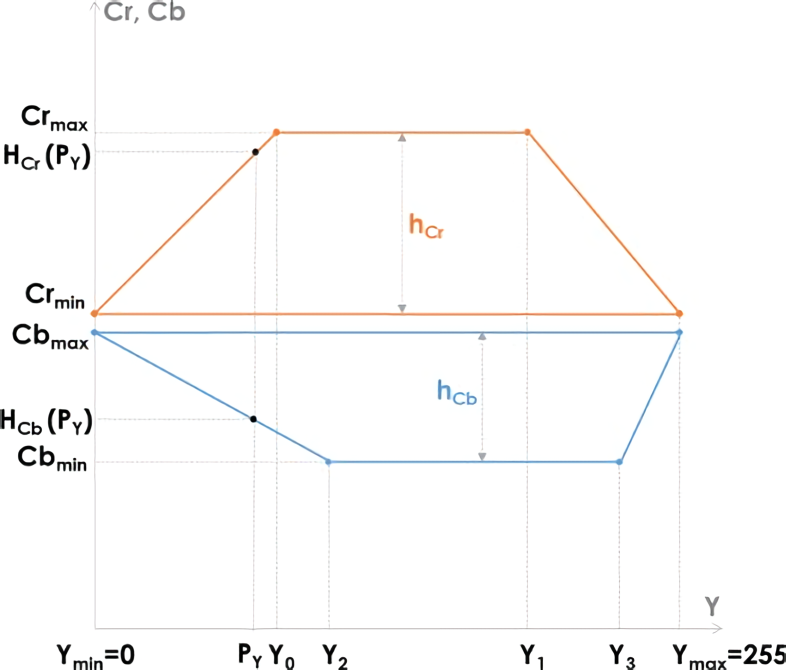
\includegraphics[width=0.6\linewidth]{images/approaches/thresholding/trapezia_other_sides.png}
	\caption{Graphical representation of $T_{YCr}$ and $T_{YCb}$. Adapted from Brancati \textit{et al.} 2017~\cite{brancati2017human}.}
	\label{fig:trapeze-other-sides}
\end{figure}

\begin{figure}[!htb]
	\centering
	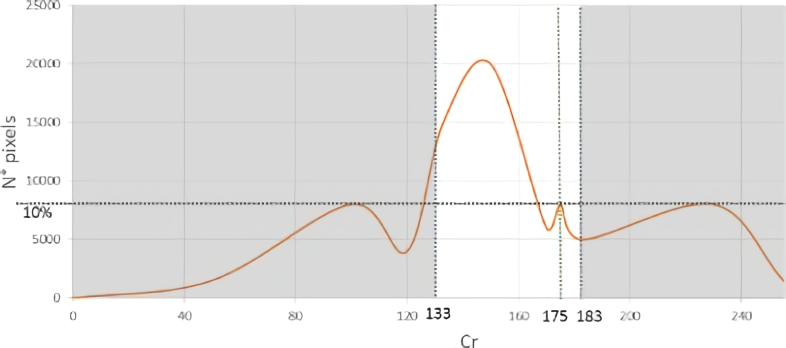
\includegraphics[width=0.9\linewidth]{images/approaches/thresholding/dyc_percentile.png}
	\caption{Computation of $Cr_{max}$ on the histogram of Cr values. Adapted from Brancati \textit{et al.} 2017~\cite{brancati2017human}.}
	\label{fig:dyc-percentile}
\end{figure}

The correlation rules between the chromatic components $P_{Cr}$ and $P_{Cb}$ of a pixel $P$ are defined by the computation of some parameters, as follows:

\begin{equation}
\begin{aligned}
&P_{C r}-P_{C b} \geq I_{P} \\
\end{aligned}
\end{equation}

\begin{equation}
\begin{aligned}
&\left|P_{C b}-P_{C b_{s}}\right| \leq J_{P}\\
\end{aligned}
\end{equation}

where $I_P$ is the minimum difference between the values $P_{Cr}$ and $P_{Cb}$, $P_{C b_{s}}$ is an estimated value of $P_{Cb}$, and $J_P$ is the maximum distance between the points $(P_Y, P_{Cb})$ and $(P_Y, P_{C b_{s}})$.

\noindent A pixel $P$ is classified as a skin pixel if both the conditions hold. The first rule indicates that the chrominance components should be sufficiently far from each other.
The second represents the range of values delimiting the $P_{C b_{s}}$ value, to which the $P_{Cb}$ should belong. \autoref{fig:trapeze-params} gives a visual representation of the operations to perform to compute the required parameters.

\begin{figure}[h]
	\centering
	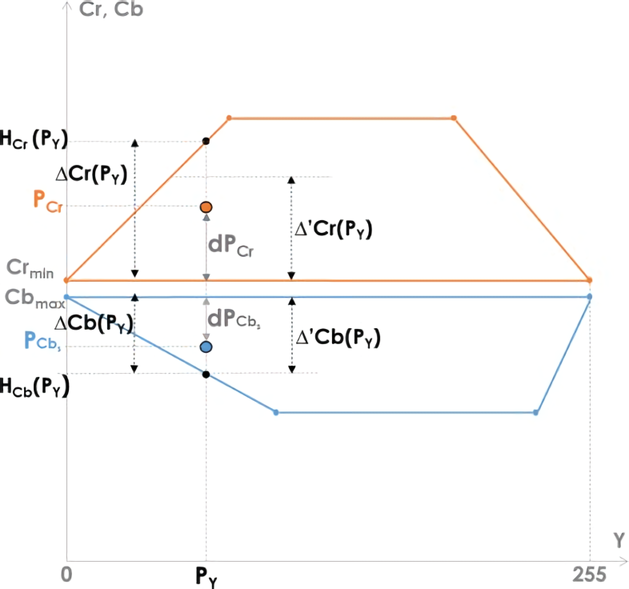
\includegraphics[width=0.6\linewidth]{images/approaches/thresholding/trapezia_params.png}
	\caption{Computation of the correlation rules parameters. Adapted from Brancati \textit{et al.} 2017~\cite{brancati2017human}.}
	\label{fig:trapeze-params}
\end{figure}

\begin{equation}
\begin{aligned}
P_{C b_{s}} = Cb_{max} - dP_{C b_{s}}\\
P_{Cr} = Cr_{min} + dP_{Cr}
\end{aligned}
\end{equation}

with $dP_{C b_{s}}$ and $dP_{Cr}$ as the distances respectively between the points $(P_Y, P_{C b_{s}})$ and $(P_Y, P_{Cr})$, and the longer bases of the trapezium in the corresponding subspaces.
It is possible to compute $dP_{C b_{s}}$ with respect to $dP_{Cr}$ on the basis of the inversely proportional behavior of the chrominance components observed within the trapezium:

\begin{equation}
\begin{aligned}
dP_{C b_{s}} = \alpha \cdot dP_{Cr}
\end{aligned}
\end{equation}

where $\alpha$ takes into account the different shapes of the trapezium, being computed as the ratio between the normalized heights of the two trapeziums in correspondence with the current luminance value $P_Y$ as follows:

\begin{equation}
\begin{aligned}
\Delta_{Cr}(P_Y) = H_{Cr}(P_Y) - Cr_{min}\\
\Delta_{Cb}(P_Y) = Cb_{max} - H_{Cb}(P_Y)
\end{aligned}
\end{equation}

where $\Delta_{Cr}(P_Y)$ and $\Delta_{Cb}(P_Y)$ represent the distances between the points $(P_Y, H_{Cr}(P_Y))$ and $(P_Y, H_{Cb}(P_Y))$ and the longer base of their respective trapezium.

\noindent Now, the values of $\Delta_{Cr}(P_Y)$ and of $\Delta_{Cb}(P_Y)$ are normalized with respect to the difference in the size of the trapeziums:

\begin{equation}
\begin{aligned}
&\Delta_{C r}^{\prime}\left(P_{Y}\right)=\left\{\begin{array}{ll}
\Delta_{C r}\left(P_{Y}\right) \cdot \frac{A_{T_{YCb}}}{A_{T_{YCr}}} & \text { if } A_{T_{YCr}} \geq A_{T_{YCb}} \\
\Delta_{C r}\left(P_{Y}\right) & \text { otherwise }
\end{array}\right. \\ \\
&\Delta_{C b}^{\prime}\left(P_{Y}\right)=\left\{\begin{array}{ll}
\Delta_{C b}\left(P_{Y}\right) & \text { if } A_{T_{YCr}} \geq A_{T_{YCb}} \\
\Delta_{C b}\left(P_{Y}\right) \cdot \frac{A_{T_{YCr}}}{A_{T_{YCb}}} & \text { otherwise }
\end{array}\right.
\end{aligned}
\end{equation}

where $A_{T_{YCr}}$ and $A_{T_{YCb}}$ are the areas of the trapeziums $T_{YCr}$ and $T_{YCb}$, respectively.
Then, the value $\alpha$ is given by:

\begin{equation}
\begin{aligned}
\alpha=\frac{\Delta_{C b}^{\prime}\left(P_{Y}\right)}{\Delta_{C r}^{\prime}\left(P_{Y}\right)}\\
\end{aligned}
\end{equation}

\noindent Finally, the remaining parameters $I_P$ and $J_P$ are given by:

\begin{equation}
\begin{aligned}
I_{P}=s f \cdot\left[\left(\Delta_{C r}^{\prime}(Y)-d P_{C r}\right)+\left(\Delta_{C b}^{\prime}(Y)-d P_{C b_{s}}\right)\right]
\\ \\
J_{P}=d P_{C b_{s}} \cdot \frac{d P_{C b_{s}}+d P_{C r}}{\Delta_{C b}^{\prime}(Y)+\Delta_{C r}^{\prime}(Y)}
\\ \\
s f=\frac{\min \left(\left(Y_{1}-Y_{0}\right),\left(Y_{3}-Y_{2}\right)\right)}{\max \left(\left(Y_{1}-Y_{0}\right),\left(Y_{3}-Y_{2}\right)\right)}
\end{aligned}
\end{equation}


\FloatBarrier
%%%%%%%%%%%%%%%%%%%%%%%%%%%%%%%%%%%%%%%%%%%%%%%%%%%%%%%%%%%%%%%%%%%%%%%%
\section{Statistical}
%%%%%%%%%%%%%%%%%%%%%%%%%%%%%%%%%%%%%%%%%%%%%%%%%%%%%%%%%%%%%%%%%%%%%%%%

Large amount of data can support simple and computationally efficient learning algorithms~\cite{jones2002statistical}.
Statistical methods aim at creating a model to understand how the data are related in order to make predictions (an example can be seen in \autoref{fig:statistical-model-example}).
When performing classification, these models not only allow to predict the class label, but also to obtain a probability of the respective label.
This probability gives the confidence on the prediction.

Given a probability, different rules can be used to perform the classifications, with one of the most common being the Bayes rule.
In binary classification problems, a single threshold is involved to choose at which probability one class should be classified over another.
The thresholding rule is not unique, multiple rules have been used in the literature~\cite{jones2002statistical, phung2001universal}.

% IN SKIN DETECTION
In skin detection, one of the most popular work of statistical modeling has been published in 2002~\cite{jones2002statistical}: a Bayesian classifier has been used to perform classifications starting from the probabilities given by statistical models.
In the same work, skin and non-skin gaussian mixture models using a parallel implementation of the standard EM algorithm~\cite{redner1984mixture} and $16$ gaussians in each model have been trained.
A comparison with histogram models of size $32$ is presented.
The results describe slightly better performance in the case of the histogram models, which also took only a matter of minutes to train, as opposed to about $24$ hours required by the gaussian mixture models.
A mixture model is also slower to use during classification since all the gaussians must be evaluated in computing the probability of a single color value.
Contrarily, a histogram model translates to a fast classifier since only two table lookups are required to compute the probability of skin.
However, from a storage point of view, the gaussian mixture models are much more compact: $896$ bytes in contrast to $262$ Kbytes of the histogram models.\\
Gomez \textit{et al.} 2002~\cite{gomez2002selecting} presented a work in which two 3-dimensional histogram models are constructed to represent the skin and non-skin classes, and the probability is computed with a rule different than the Bayes theorem.

\begin{figure}[h]
    \centering
    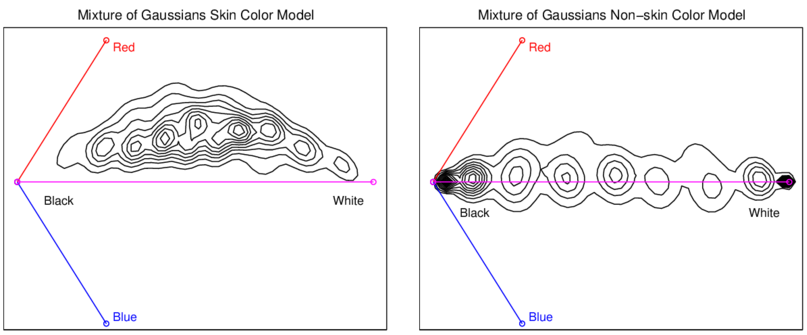
\includegraphics[width=0.9\linewidth]{images/approaches/statistical/statistical_model.png}
    \caption{Mixture of gaussians are an example of statistical models.
    Adapted from Jones and Rehg 2002~\cite{jones2002statistical}}
    \label{fig:statistical-model-example}
\end{figure}


\FloatBarrier
%%%%%%%%%%%%%%%%%%%%%%%%%%%%%%%%%%%%%%%%%%%%%%%%%%%%%%%%%%%%%%%%%%%%%%%%
\subsection{Implementation}\label{sec:impl-bayes}
%%%%%%%%%%%%%%%%%%%%%%%%%%%%%%%%%%%%%%%%%%%%%%%%%%%%%%%%%%%%%%%%%%%%%%%%

%% SPIEGO MODELLO SCELTO
The chosen implementation\footnote{Source code available at \url{https://github.com/Chinmoy007/Skin-detection}}\ uses three-dimensional histograms to model the data and probability calculus to perform the classification~\cite{acharjee2018skin}.
The training data is used to construct two histogram models representing the probabilities of skin and non-skin classes, with RGB as the color space and a histogram size of $256$ bins per color component.
The models are saved as a lookup table.
The thresholding value utilized to label skin pixels is $0.555555$.\\
An overview of the algorithm is presented below:
\vspace{5mm}

\begin{minipage}{\linewidth}%
\noindent Training:
    \begin{enumerate}[Step 1:]
    \item Initialize two 3-dimensional data structures
    \item Pick an image and the corresponding mask from the training dataset
    \item Loop every (R,G,B) pixel of the image
    \item Pick the corresponding pixel from the mask: if it is a skin pixel, increase the value at position [R, G, B] of the data structure representing skin, otherwise increase the value in the other structure
    \item Return to the first step until the training images have all been processed 
    \end{enumerate}
    
    \vspace{3mm}
    \noindent Predicting:
    \begin{enumerate}[Step 1:]
    \item Loop every (R,G,B) pixel from input image
    \item Calculate the probability of that (R,G,B) color combination of being skin
    \item If skin probability > $\Theta$, the pixel is classified as skin
    \end{enumerate}
\end{minipage}

\vspace{7mm}
\noindent The key step in skin pixel classification is the computation of $P (skin \mid rgb)$, which is the probability of a given $rgb$ pixel to belong to the skin class, and it is given by the following rule:

\begin{equation}
    P(skin \mid rgb) = \frac{s[rgb]}{s[rgb] + n[rgb]}
\end{equation}

where $s[rgb]$ is the pixel count contained in bin $rgb$ of the skin histogram and $n[rgb]$ is the equivalent count from the non-skin histogram.\\
% threshold
A particular RGB value is labeled skin if:

\begin{equation}
\label{eqn:bayes-thresh}
P(s k i n \mid r g b) \geq \Theta
\end{equation}

where  $0 \leq \Theta \leq 1 $ is a threshold value that can be adjusted to trade-off between true positives and false positives.

\noindent It is important to note that using color spaces other than RGB (such as YCBCr or HSV) will not improve the performance of the skin detector~\cite{jones2002statistical}.
The Detector performance depends entirely on the amount of overlap between the skin and non-skin samples. Colors that occur in both classes with comparable frequencies cannot be classified reliably.


%% HISTOGRAM MODEL DESCRIPTION - SPIEGO DETTAGLIATO
There are different ways to build the skin and non-skin color models.
One of the most common is to utilize \textbf{histogram models}: the skin and non-skin pixels contained in the training set images are placed into the skin and non-skin histograms, respectively.\\
Before constructing an histogram model, two requirements are needed: a color space and the size of the histogram, which is measured by the number of bins per color channel.
The fact that the performance of the classifier is independent of the color space, and RGB being the most common and natural color space used in image representation, makes RGB the favorite choice.
Color images usually store $24$ bits for each pixel, as there are three color components represented by $8$ bits each. Each color component is thereby able to represent $2^8=256$ levels of intensity.

\begin{figure}[h]
     \centering
     \begin{subfigure}[b]{0.45\textwidth}
         \centering
         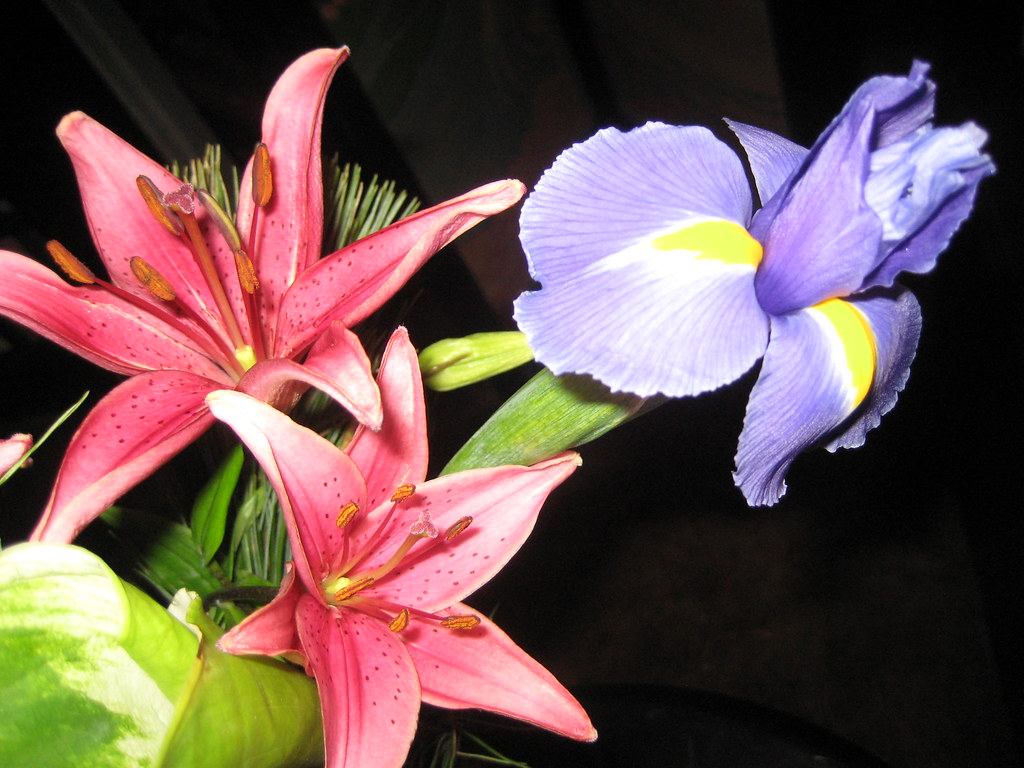
\includegraphics[width=\textwidth]{images/approaches/statistical/3d-hist-orig.jpg}
         \caption{}
         \label{fig:3d-hist-orig}
     \end{subfigure}
     \hfill
     \begin{subfigure}[b]{0.45\textwidth}
         \centering
         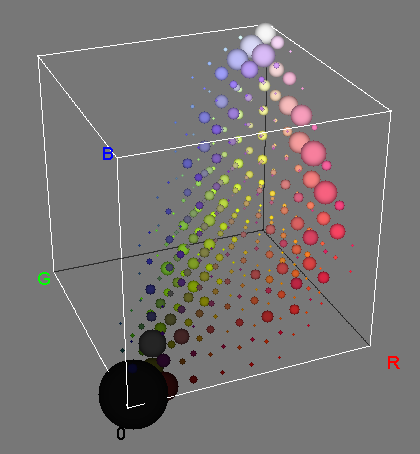
\includegraphics[width=\textwidth]{images/approaches/statistical/3d-hist-plug.png}
         \caption{}
         \label{fig:3d-hist-plug}
     \end{subfigure}
        \caption[footnote-3d]{3D histogram representation: (a) original photo by Jose and Roxanne licensed under CC BY 2.0; (b) visualization made utilizing the \q{3D Color Inspector} plugin of ImageJ.\footnotemark}
        \label{fig:3d-hist}
\end{figure}
\footnotetext{Plugin available at \url{https://imagej.nih.gov/ij/plugins/color-inspector.html}} % Anywhere on the same page where the float appears - TODO

When building the histogram, the number of bins is important. Too few bins could result in poor accuracy, while too many bins could lead to over-fitting~\cite{jones2002statistical}.
Reducing the number of bins helps to \q{generalise} and compact the histogram~\cite{gomez2002selecting}.
By using fewer bins, a set of points of similar color is represented by a single color (this technique is called color quantization. An example of a 3D histogram using the technique is depicted in \autoref{fig:3d-hist}).
By using a $24$-bit pixel representation, the histogram model would have a size of $256$ bins per color channel, which correspond to more than 16 million ($256^3$) bins, each mapped to a specific (R,G,B) color triple.
Jones and Rehg (2002)~\cite{jones2002statistical} found the best histogram size in their experiments to be $32$.
They also reported that, with a histogram size of $256$, $77\%$ of the possible $24$-bit RGB colors are never encountered, and thus the histogram is mostly empty.\\
Using a histogram size of $256$ in the RGB color space means that each of the three histogram dimensions is divided into $256$ bins. And each bin stores an integer counting the number of times that color value occurred in the entire database of images.


\FloatBarrier
%%%%%%%%%%%%%%%%%%%%%%%%%%%%%%%%%%%%%%%%%%%%%%%%%%%%%%%%%%%%%%%%%%%%%%%%
\section{Convolutional Neural Networks}
%%%%%%%%%%%%%%%%%%%%%%%%%%%%%%%%%%%%%%%%%%%%%%%%%%%%%%%%%%%%%%%%%%%%%%%%

Convolutional Neural Networks (CNNs) are a type of Neural Network commonly applied to analyze visual scenes. Their structure is inspired by the human brain, mimicking the way that biological neurons signal to one another.


\FloatBarrier
%%%%%%%%%%%%%%%%%%%%%%%%%%%%%%%%%%%%%%%%%%%%%%%%%%%%%%%%%%%%%%%%%%%%%%%%
\subsection{Neural Networks}
%%%%%%%%%%%%%%%%%%%%%%%%%%%%%%%%%%%%%%%%%%%%%%%%%%%%%%%%%%%%%%%%%%%%%%%%

A \textbf{biological neuron} has specialized protrusions called dendrites and axons.
Dendrites bring information to the cell body, and axons take information away from the cell body.
Information flows from one neuron to another across a small gap between them named synapse.
The dendrites carry the signal to the cell body where they all get summed; if the final sum is above a certain threshold, the neuron can fire, sending a spike along its axon.

\begin{figure}[h]
	\centering
	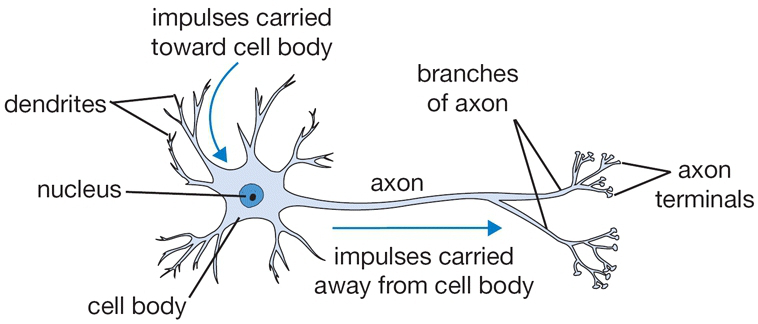
\includegraphics[width=0.7\linewidth]{images/approaches/deep_learning/neuron_b.png}
	\caption[footnote-3d]{Biological neuron.\footnotemark}
	\label{fig:neuron-bio}
\end{figure}
\footnotetext{The figure is adapted from \url{https://cs231n.github.io/neural-networks-1/}}

In the \textbf{computational model of a neuron}, also named Perceptron, the signals that travel along the axons $x_i$ interact multiplicatively $(w_ix_i)$ with the dendrites of the other neuron based on the synaptic strength $w_i$ at that synapse.
The dendrites bring the signals to the cell body, where they all get summed. The idea is that the synaptic strengths (the weights $w$) are learnable and control the strength of influence of one neuron on another. 
The neuron then performs a transformation to the input through the activation function $f(x)$ and generates the output $y$.
The activation function is typically a non-linear transformation that is applied to the input data.
The bias value $b$ allows the activation function to be shifted to the left or right, to better fit the data.
The weights and biases represent the parameters of the network.

\begin{figure}[htbp]
  \centering
  \includesvg[width=0.7\linewidth]{images/approaches/deep_learning/neuron_c.svg}
  \caption{Neuron computational model.}
  \label{fig:neuron-comp}
\end{figure}

A \textbf{Neural Network} is a group of multiple neurons connected together, as shown in \autoref{fig:forward-prop}.
Neurons are typically organized into different layers.
Neurons of one layer connect only to neurons of the immediately preceding and immediately following layers, therefore the output of a layer becomes the input of the next layer.
The first layer is the input layer, where each neuron represents a feature in the dataset, the last layer is the output layer, and all the other layers are the hidden layers.
Although a single output is depicted in the figure, the output layer can have different sizes. It can vary from one output for a single class classification to thousands of pixels of an image classification map.

\begin{figure}[h]
	\centering
	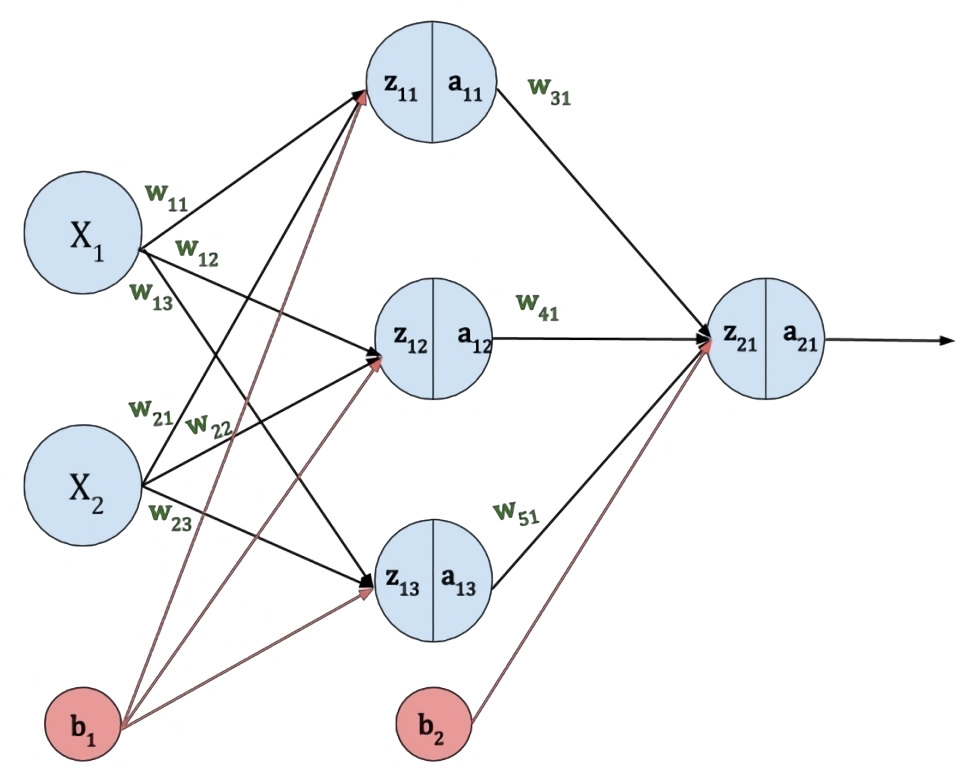
\includegraphics[width=0.7\linewidth]{images/approaches/deep_learning/forwardpass.jpg}
	\caption[footnote-3d]{A two-layer Neural Network architecture. Conventionally, the input layer is not counted for defining the number of layers of a Neural Network.
	There are two input features: $x_1$ and $x_2$, a hidden layer with three neurons, and an output layer with one neuron.
	Each neuron has assigned the weight parameter $W_{ij}$. The $b_1$ and $b_2$ are the bias parameters for the input layer and hidden layer, respectively.}
	\label{fig:forward-prop}
\end{figure}

\noindent Once the dataset and problem are defined, the main steps to train a Neural Network are the following:
\begin{enumerate}[Step 1:]
\item Construct the network architecture and initialize with random weights
\item Do a forward pass (Forward propagation)
\item Calculate the total error, which needs to be minimized
\item Back propagate the error and Update weights
\item Repeat the steps(2-4) for No. of epochs/until error is minimum.
\end{enumerate}

\noindent In \textbf{forward propagation}, the input data is fed to the network in the forward direction: each hidden layer gets the data, perform calculation and pass the result to the next layer.
Finally, the output layer calculates the output of the model.\\
The forward propagation for the network in \autoref{fig:forward-prop} is described below.
The input is represented by $X$, which can be imagined as a matrix of 2 rows and 1 column.
The next layer is represented by $z_{11}$, $z_{12}$, $z_{13}$, which are the values of the intermediate neurons calculated from the weight, bias, and neuron values of the previous layer.
This layer can be imagined as a matrix of 3 rows and 1 column.
In this case, there are two input nodes and three output nodes that the parameters must fit. $W_{\text {pln, nln }}^{\text {(layer) }}$ is the parameter to be optimized, in which $pln$ and $nln$ represent the previous layer input neuron and the next layer output neuron, respectively.
The bias parameter for the input layer is represented by $b_1$.

\begin{equation}
\begin{aligned}
{\left[\begin{array}{l}
z_{11} \\
z_{12} \\
z_{13}
\end{array}\right]=\left[\begin{array}{ll}
w_{11} & w_{21} \\
w_{12} & w_{22} \\
w_{13} & w_{23}
\end{array}\right]\left[\begin{array}{l}
x 1 \\
x 2
\end{array}\right]+\left[\begin{array}{l}
b_{1} \\
b_{1} \\
b_{1}
\end{array}\right]} \\
Z^{[1]}=W^{[1]} X+b^{[1]}
\end{aligned}
\end{equation}

\noindent An activation function $\sigma(Z)$ will be applied to the intermediate neuron values to learn the non-linear patterns between inputs and target output variables.
The $a_{11}$, $a_{12}$, and $a_{13}$ values are the output of the activation function that is applied to $z_{11}$, $z_{12}$ and $z_{13}$, respectively.

\begin{equation}
\begin{aligned}
\left[\begin{array}{l}
a_{11} \\
a_{12} \\
a_{13}
\end{array}\right] &=\sigma\left[\begin{array}{l}
z_{11} \\
z_{12} \\
z_{13}
\end{array}\right] \\
A^{[1]} &=\sigma\left(Z^{[1]}\right)
\end{aligned}
\end{equation}

\noindent At the next step, $A^{[1]}$ becomes the input layer and $z_{21}$ becomes the output layer.
There are three input nodes and an output node that the parameters must fit, so $W^{[2]}$ is a matrix with one row and three columns.
The bias parameter for the hidden layer is represented by $b_2$.

\begin{equation}
\begin{gathered}
{\left[z_{21}\right]=\left[\begin{array}{lll}
w_{31} & w_{41} & w_{51}
\end{array}\right]\left[\begin{array}{l}
a 11 \\
a 12 \\
a 13
\end{array}\right]+\left[b_{2}\right]} \\
Z^{[2]}=W^{[2]} A^{[1]}+b^{[2]}
\end{gathered}
\end{equation}

\noindent The activation function $\sigma(Z)$ is applied to the obtained values, and the algorithmic step represented by this layer finishes.

\begin{equation}
\begin{aligned}
&{\left[a_{21}\right]=\sigma\left[z_{21}\right]} \\
&A^{[2]}=\sigma\left(Z^{[2]}\right)
\end{aligned}
\end{equation}

\noindent The output of the neural network is calculated, hence the forward propagation algorithm ends.

\textbf{Activation functions} are an important part of Neural Networks.
Without them, the networks are just the weighted sum of their inputs plus a bias term, unable to learn any complex and nonlinear function.
Activation functions are means to introduce non-linearity to the model.
There are different classes of activation functions available, with common ones being the Sigmoid, the ReLU, the Tanh, and the Linear activation functions.
The mentioned activation functions are illustrated in \autoref{fig:activation-functions}.

\begin{figure}[h]
	\centering
	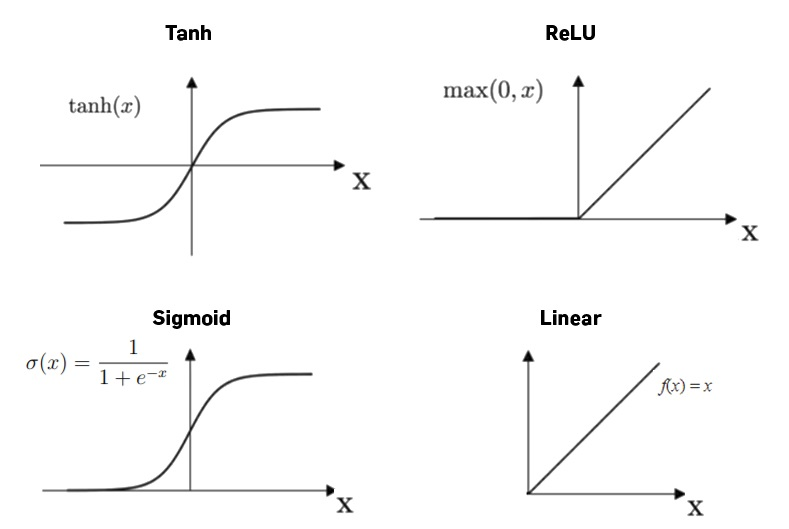
\includegraphics[width=0.9\linewidth]{images/approaches/deep_learning/activation_functions_f.jpg}
	\caption{Common activation functions. The Tanh function forces the values to be between $-1$ and $1$. The Sigmoid function forces the values to be between $0$ and $1$. The ReLU function cuts values below zero. The Linear activation function returns the input.}
	\label{fig:activation-functions}
\end{figure}

The next step in a Neural Network is to \textbf{compute the loss (error)}. Once the output of the network is obtained, it is compared to the desired output value (the so-called ground truth), and a loss function computes the error signal, which measures how well the network predicts outputs.\\
A popular loss function is the Cross-Entropy Loss, defined as follows:

\begin{equation}
\begin{aligned}
&J=-\frac{1}{m} \sum_{i=1}^{m} L\left(a^{[2](i)}, y^{(i)}\right) \\
&L\left(a^{[2]}, y\right)=-y \log a^{[2]}-(1-y) \log \left(1-a^{[2]}\right)
\end{aligned}
\end{equation}

where L is the loss function and J is the cost function: the average loss over the entire training dataset.

\noindent The goal is to then find a set of weights and biases that minimizes the error.
However, it is impossible to compute the error signal for internal neurons directly because the output values of these neurons are unknown.
The idea is to propagate the error signal back to all neurons by computing the gradient of the loss function with respect to each weight.
The derivative of the loss function on each parameter gives information about how changing the parameter impacts the function value.
The algorithm that computes the gradient is called \textbf{backpropagation}.

\begin{figure}[h]
	\centering
	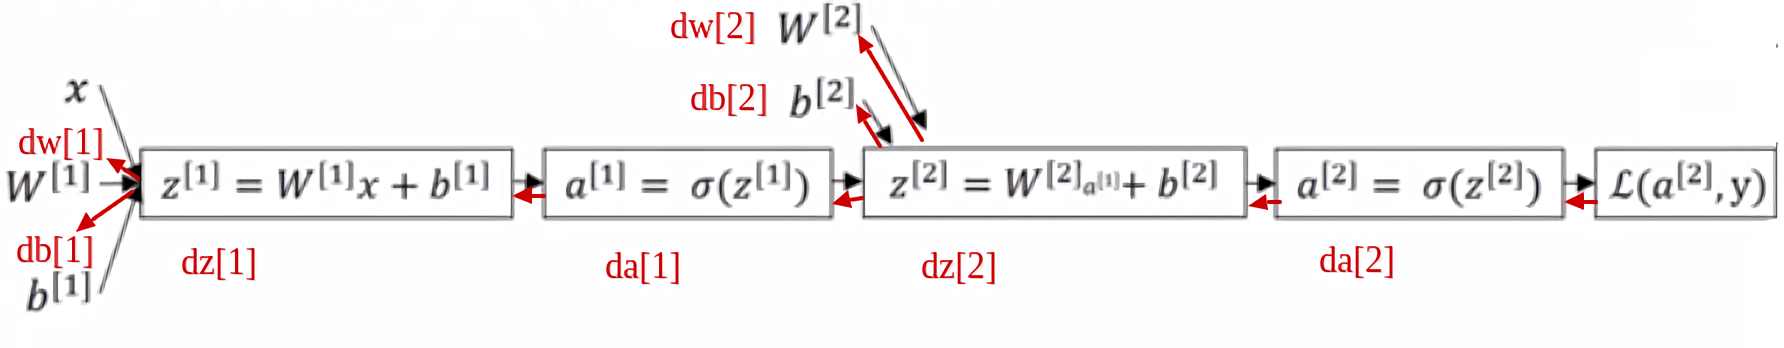
\includegraphics[width=0.9\linewidth]{images/approaches/deep_learning/backprop_nn.png}
	\caption[footnote-3d]{The red line represents the back-propagation process. The $da[2]$, $dz[2]$, $dw[2]$, $db[2]$, $da[1]$, $dz[1]$, $dw[1]$ and $db[1]$ are the partial derivative of the loss function with respect to $a[2]$, $z[2]$, $w[2]$, $b[2]$, $a[1]$, $z[1]$, $w[1]$ and $b[1]$ respectively.}
	\label{fig:backprop}
\end{figure}

While performing the derivative calculation, it is also necessary to calculate the derivative of the activation function. Below is presented the derivative of the Sigmoid Activation function:

\begin{equation}
\begin{aligned}
\sigma(x) &=\frac{1}{1+e^{-x}}=\left(1+e^{-x}\right)^{-1} \\
\sigma^{\prime}(x) &=\left(1+e^{-x}\right)^{-2} e^{-x} \\
&=\frac{e^{-x}}{\left(1+e^{-x}\right)^{2}} \\
&=\frac{1}{\left(1+e^{-x}\right)} * \frac{1+e^{-x}-1}{\left(1+e^{-x}\right)} \\
&=\frac{1}{\left(1+e^{-x}\right)} *\left(1-\frac{1}{1+e^{-x}}\right) \\
&=\sigma(x)(1-\sigma(x))
\end{aligned}
\end{equation}

\noindent The computation of the partial derivative of weight and bias parameters is done as follows:

\begin{align}
d a^{[2]}&=\frac{\partial L}{\partial a^{[2]}} & d a^{[1]}&=\frac{\partial L}{\partial a^{[1]}} \nonumber\\
d z^{[2]}&=\frac{\partial L}{\partial z^{[2]}} & d z^{[1]}&=\frac{\partial L}{\partial z^{[1]}} \nonumber\\
d w^{[2]}&=\frac{\partial L}{\partial w^{[2]}} & d w^{[1]}&=\frac{\partial L}{\partial w^{[1]}} \nonumber\\
d b^{[2]}&=\frac{\partial L}{\partial b^{[2]}} & d b^{[1]}&=\frac{\partial L}{\partial b^{[1]}} 
\end{align}

\noindent When the error signal for each neuron is computed, the weights coefficients of each neuron input node may be modified to minimize the error.
The \textbf{weight updating} is commonly performed by a gradient descent algorithm, which takes advantage of the already calculated gradients.
The weight and bias parameters are updated by subtracting the partial derivative of the loss function with respect to those parameters.
A visualization of the gradient descent algorithm is displayed in \autoref{fig:grad-descent}.
The step size can be modified accordingly thanks to the learning rate coefficient $\alpha$, which controls how much to update the parameter.

\begin{equation}
\begin{aligned}
W^{[1]}=W^{[1]}-\alpha \frac{\partial L}{\partial W^{[1]}}\\
b^{[1]}=b^{[1]}-\alpha \frac{\partial L}{\partial b^{[1]}}\\
W^{[2]}=W^{[2]}-\alpha \frac{\partial L}{\partial W^{[2]}}\\
b^{[2]}=b^{[2]}-\alpha \frac{\partial L}{\partial b^{[2]}}
\end{aligned}
\end{equation}

\begin{figure}[!htb]
	\centering
	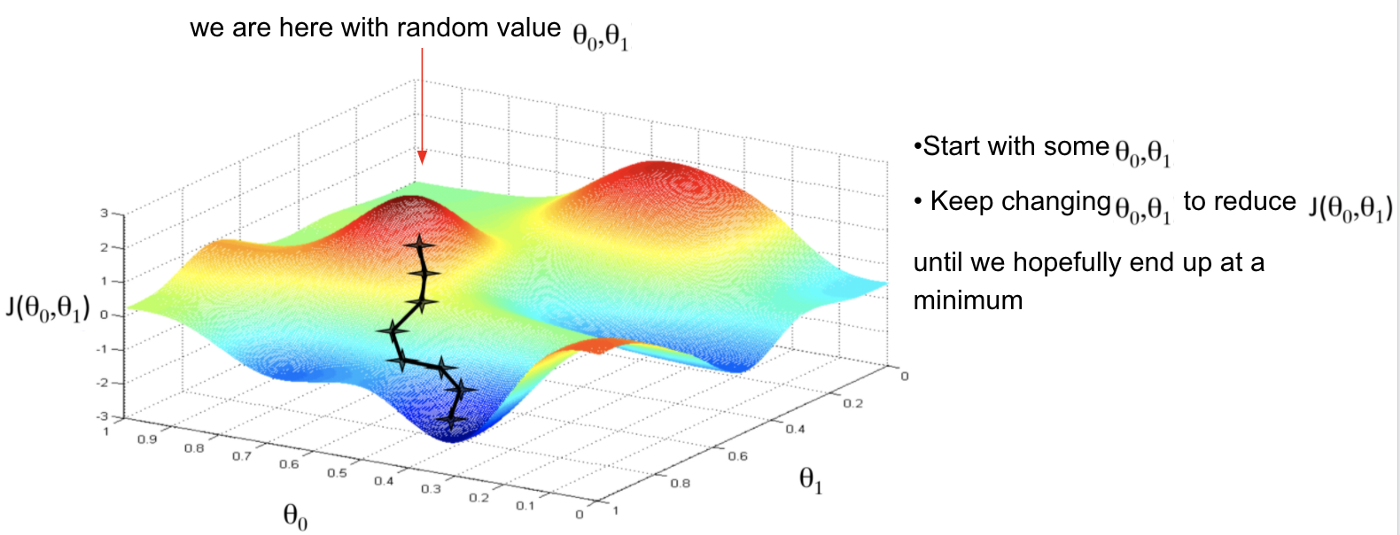
\includegraphics[width=0.9\linewidth]{images/approaches/deep_learning/grad_descent.png}
	\caption{Visualization of the gradient descent algorithm. $\theta_0$ and $\theta_1$ represent the parameters to update: the bias and the weight values, respectively.}
	\label{fig:grad-descent}
\end{figure}


\FloatBarrier
%%%%%%%%%%%%%%%%%%%%%%%%%%%%%%%%%%%%%%%%%%%%%%%%%%%%%%%%%%%%%%%%%%%%%%%%
\subsubsection*{Convolutions in Neural Networks}
%%%%%%%%%%%%%%%%%%%%%%%%%%%%%%%%%%%%%%%%%%%%%%%%%%%%%%%%%%%%%%%%%%%%%%%%

A Convolutional Neural Network (CNN) has the same architecture as the usual Neural Network but arranges its neurons in three dimensions (width, height, depth). Every layer of a CNN transforms the 3D input volume to a 3D output volume of neuron activations.
There are three typologies of layers utilized in a CNN architecture: the convolutional layer, which increases the efficiency of the forward function and vastly reduces the number of parameters, the pooling layer, and the fully-connected layer, which is the regular layer present in Neural Networks.
Typically convolutional layers are followed by an activation function, such as a ReLU.
The convolutional and pooling layers are used for feature extraction, while the fully connected layers are used for classification. An architecture overview is displayed in \autoref{fig:cnn-arch}.

\begin{figure}[h]
	\centering
	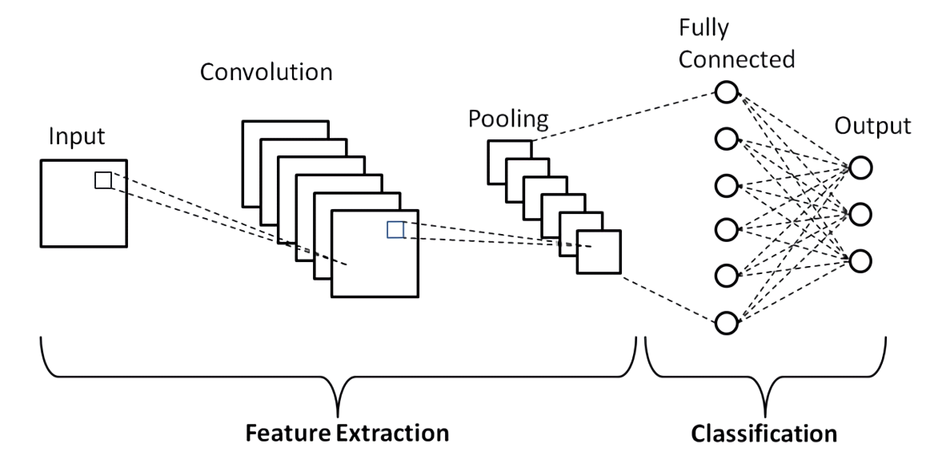
\includegraphics[width=0.9\linewidth]{images/approaches/deep_learning/cnn_arch.png}
	\caption{Overview of a CNN architecture.}
	\label{fig:cnn-arch}
\end{figure}

The \textbf{Convolutional layer}’s parameters consist of a set of learnable filters. Every filter is small spatially (along width and height) but extends through the full depth of the input volume.
A typical filter on the first layer of a Convolutional Neural Network might have size 5x5x3 because colored images have depth 3, the color channels.
During the forward pass, each filter is slid across the width and height of the input volume. The dot products between the entries of the filter and the input at any position are computed.
As the filter slides over the width and height of the input volume, it produces a 2-dimensional activation map that represents the responses of that filter at every spatial position.
In this way, the network will learn filters that activate when they see some type of visual features, such as an edge.
Inside a convolutional layer, there is a set of filters: each of them extracts a particular feature and produces a separate 2-dimensional activation map.
These activation maps are stacked along the depth dimension and produce the output volume.

The first advantage of a convolutional layer is the \textbf{local connectivity} (depicted in \autoref{fig:cnn-local}): each neuron of the layer is connected only to a local region of the input volume.
The spatial extent of this connectivity is a hyperparameter called the receptive field of the neuron (equivalently this is the filter size). The connections are local in 2D space (along width and height) but always full along with the entire depth of the input volume.

The second advantage is \textbf{parameter sharing}.
It is possible to dramatically reduce the number of parameters by making one reasonable assumption: if one feature is useful to compute at some spatial position (x,y), then it should also be useful to compute at a different position (x2,y2).
A practical application of this reasoning can be found in \autoref{fig:cnn-filters}.
The parameter sharing is done by slicing the depth of the volume size into 2-dimensional slices, called depth slices. The neurons in each depth slice share the same weights and bias.
For example, a volume of size 55x55x96 has 96 depth slices, each of size 55x55; by using a filter size of 11x11x3 on the volume, the convolutional layer will have only 96 unique sets of weights for a total of $96*11*11*3 = 34\,848$ unique weights, or $34\,944$ parameters (+$96$ biases).
Without this technique, the parameters would have been much more: $96*55*55 = 290\,400$ neurons, each using $11*11*3 = 363$ weights and $1$ bias, for a total of $290\,400 * 364 = 105\,705\,600$ parameters.
During backpropagation, every neuron in the volume will compute the gradient for its weights, but these gradients will be added up across each depth slice, and only update a single set of weights per slice.

\begin{figure}[!h]
     \centering
     \begin{subfigure}[b]{0.45\textwidth}
         \centering
         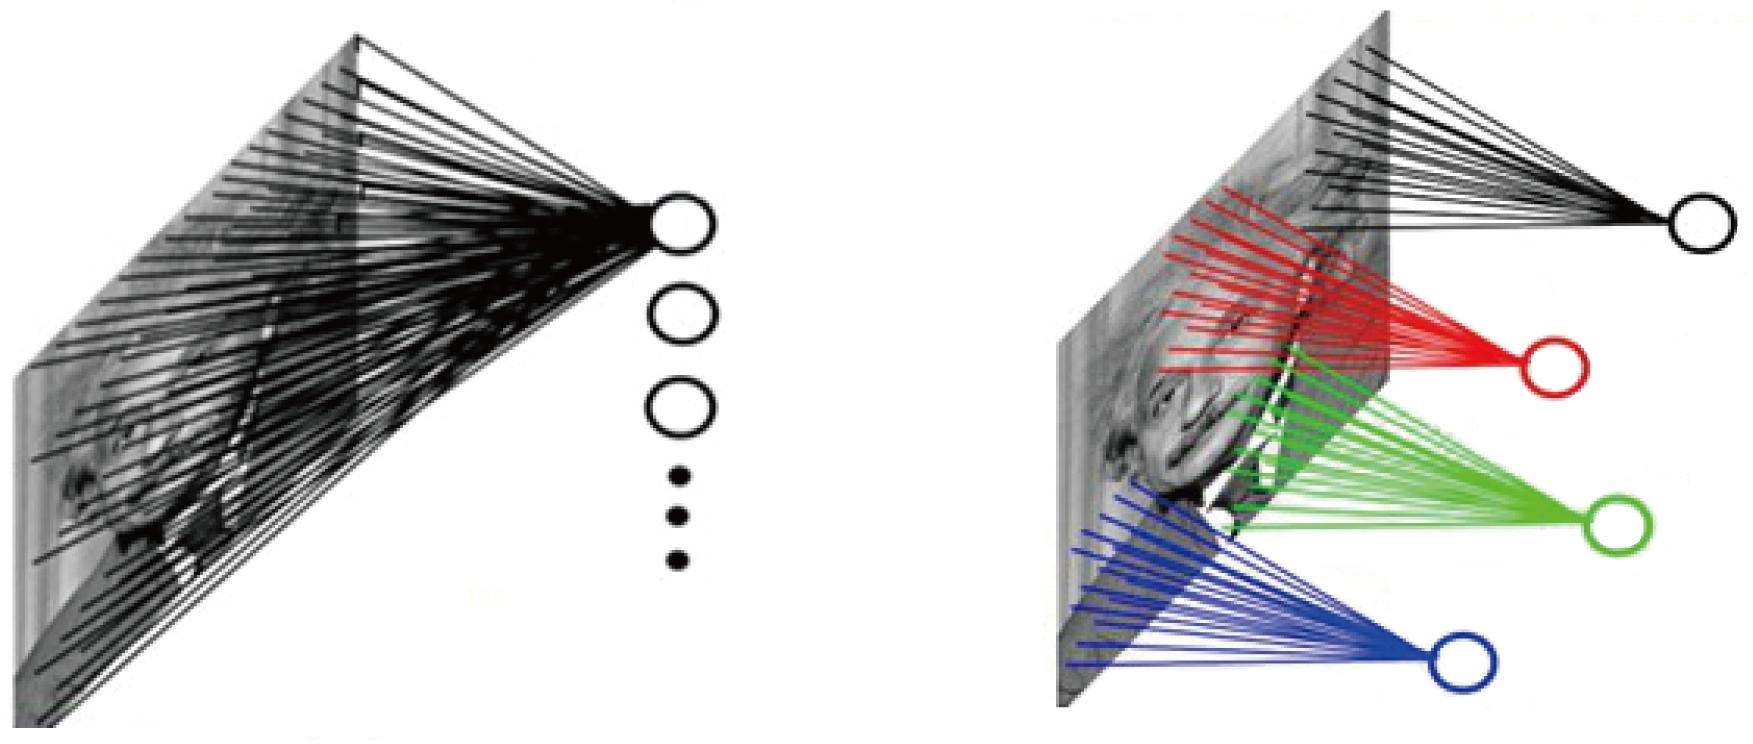
\includegraphics[width=\textwidth]{images/approaches/deep_learning/cnn_local.png}
         \caption{}
         \label{fig:cnn-local}
     \end{subfigure}
     \hfill
     \begin{subfigure}[b]{0.45\textwidth}
         \centering
         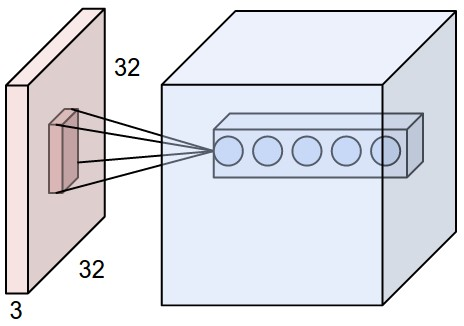
\includegraphics[width=\textwidth]{images/approaches/deep_learning/conv_filter_depth.jpeg}
         \caption{}
         \label{fig:cnn-filter-depth}
     \end{subfigure}
        \caption{Some Convolutional layer features. (a) Global (left) and local (right) perception.
        (b) The red volume represents an example input, a 32x32x3 image, and the blue volume is an example volume of neurons in the first Convolutional layer.
        Each neuron in the convolutional layer is connected only to a local region in the input volume spatially, but to the full depth (all color channels).
        Note, there are multiple neurons (5 in this example) along with the depth, all looking at the same region in the input: these neurons share the same receptive field.
        Despite this, they do not share the same weights, because they are associated with 5 different filters.}
        \label{fig:cnn-features-1}
\end{figure}

\begin{figure}[h]
	\centering
	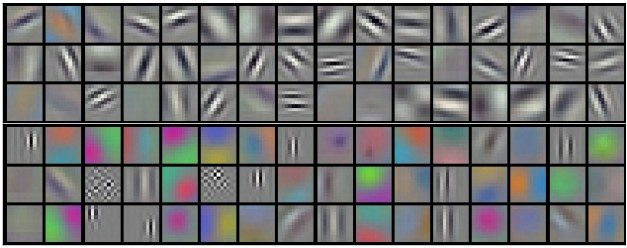
\includegraphics[width=0.9\linewidth]{images/approaches/deep_learning/filters.jpeg}
	\caption{Example filters adapted from Krizhevsky \textit{et al.} 2012~\cite{krizhevsky2012imagenet}.
	Each of the 96 filters shown here is of size [11x11x3], and each one is shared by the 55*55 neurons in one depth slice.
	Notice that the parameter sharing assumption is relatively reasonable: if detecting a horizontal edge is important at some location in the image, it should intuitively be useful at some other location as well.
	There is therefore no need to relearn to detect a horizontal edge at every one of the 55*55 distinct locations in the Conv layer output volume.}
	\label{fig:cnn-filters}
\end{figure}

It is common to periodically insert a \textbf{Pooling layer}, which performs a form of non-linear down-sampling, in-between successive Convolutional layers in a CNN architecture.
Its function is to progressively reduce the spatial size of the representation to reduce the number of parameters and computation in the network, and hence to also control overfitting.
There are several non-linear functions to implement pooling, where max pooling is the most common (depicted in \autoref{fig:max-pool}.
It partitions the input image into a set of rectangles and, for each such sub-region, outputs the maximum.
It is important to note that pooling loses the precise spatial relationships between high-level parts (such as nose and mouth in a face image).

\begin{figure}[h]
	\centering
	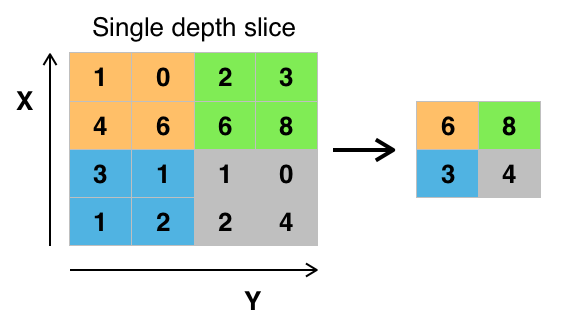
\includegraphics[width=0.7\linewidth]{images/approaches/deep_learning/Max_pooling.png}
	\caption{Max pooling with a 2x2 filter and stride = 2: the filter moves two pixels right for each horizontal movement and two pixels down for each vertical movement.}
	\label{fig:max-pool}
\end{figure}

\FloatBarrier
%%%%%%%%%%%%%%%%%%%%%%%%%%%%%%%%%%%%%%%%%%%%%%%%%%%%%%%%%%%%%%%%%%%%%%%%
\subsection{Implementation}\label{sec:impl-unet}
%%%%%%%%%%%%%%%%%%%%%%%%%%%%%%%%%%%%%%%%%%%%%%%%%%%%%%%%%%%%%%%%%%%%%%%%

%% SPIEGO MODELLO SCELTO
The chosen implementation\footnote{Source code available at \url{https://github.com/ttarasiewicz/Skinny}} consists of a modified U-Net~\cite{ronneberger2015u} incorporating dense blocks and inception modules to benefit from a wider spatial context.
The network is named Skinny~\cite{tarasiewicz2020skinny} and is depicted in \autoref{fig:skinny-arch}.
An additional deep level is appended to the original U-Net model, to better capture large-scale contextual features in the deepest part of the network.
The features extracted in the contracting path propagate to the corresponding expansive levels through the dense blocks.
The original U-Net convolutional layers are replaced with the inception modules: before each max-pooling layer, in the contracting path, and after concatenating features, in the expanding path.
Thanks to these architectural choices, Skinny benefits from a wider pixel context.

\begin{figure}[h]
	\centering
	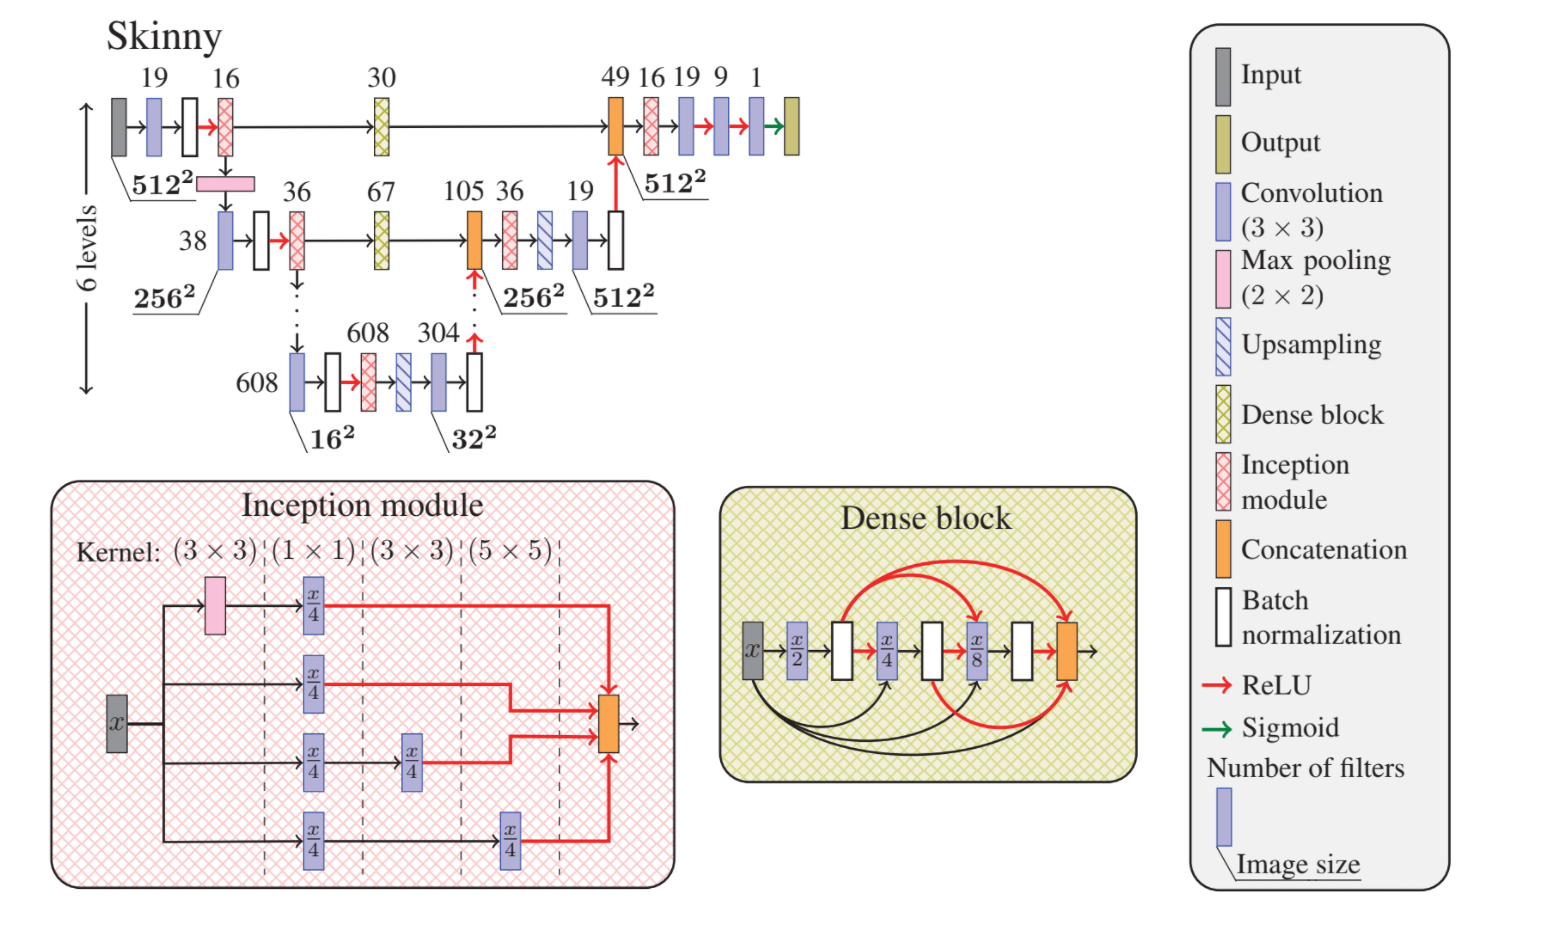
\includegraphics[width=0.9\linewidth]{images/approaches/deep_learning/skinny_arch.png}
	\caption{The architecture of Skinny.
	Adapted from Tarasiewicz \textit{et al.} 2020~\cite{tarasiewicz2020skinny}}
	\label{fig:skinny-arch}
\end{figure}


%% SPIEGO NEL DETTAGLIO
\noindent In image segmentation, it would be useful for the output of a Neural Network to be directly a classification map.
It can be achieved by decapitating the fully connected layers of a CNN network, converting it into a \textbf{Fully Convolutional Network (FCN)}~\cite{long2015fully}.
In fact, fully connected layers can be viewed as convolutions with kernels that cover their entire input regions.
An example of a fully convolutional network is the \textbf{U-Net}~\cite{ronneberger2015u} (called in this way because of its U shape, which can be seen in \autoref{fig:enc-dec}), a famous network used for semantic segmentation.
The architecture of an FCN can be seen as a union of two networks: an encoder, which takes the input and output a feature map, and a decoder, which takes the feature vector from the encoder and gives a classification map in output.

\begin{figure}[h]
	\centering
	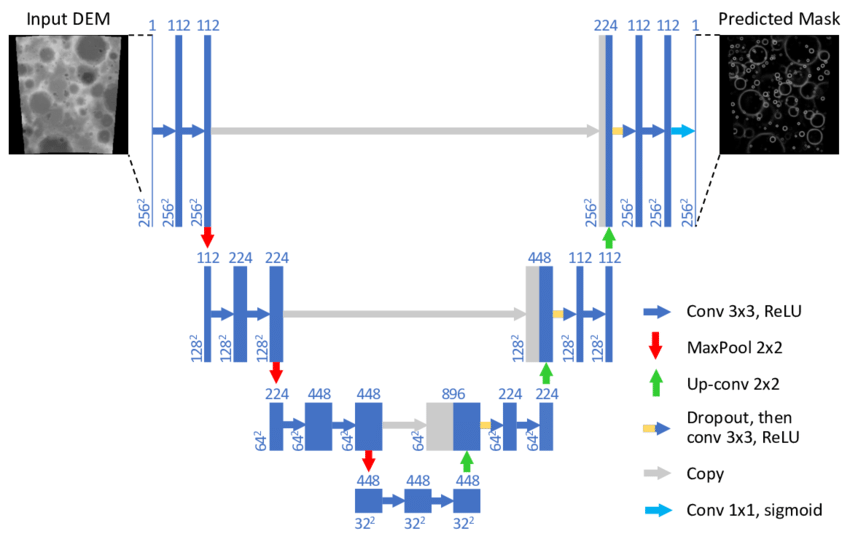
\includegraphics[width=0.9\linewidth]{images/approaches/deep_learning/unet_arch.png}
	\caption{U-Net is a Fully Convolutional Network that utilizes the encoder-decoder architecture.
	The encoder consists of the contracting pathway of the network, while the decoder consists of the expanding pathway.
	Adapted from Silburt \textit{et al.} 2019~\cite{silburt2019lunar}}
	\label{fig:enc-dec}
\end{figure}

The encoder performs the feature extraction task via multiple down-sampling operations, in the same way as the first part of a CNN.
The decoder must then up-sample these feature maps multiple times until the achievement of the desired classification map, which size is determined by the architecture.
The upsampling operation is possible thanks to the skip connections.
\textbf{Skip connections} are used to skip features from the contracting path to the expanding path in order to recover spatial information lost during downsampling, making fully convolutional methods suitable for semantic segmentation.
The \textbf{Up-sampling layer} consists of a transposed convolution, an operation that goes in the opposite direction to a convolution, as shown in \autoref{fig:deconv}.

\begin{figure}[h]
	\centering
	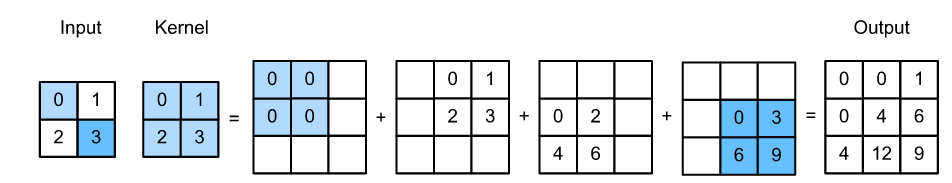
\includegraphics[width=0.9\linewidth]{images/approaches/deep_learning/deconv_w.png}
	\caption{Transposed convolution. Each element of the input feature map is taken and multiplied with every element of the kernel. The outputs of these operations are then summed.}
	\label{fig:deconv}
\end{figure}

The main advantage of the chosen implementation compared to a regular U-Net is the addition of inception modules and dense blocks.
Salient parts in the image can have extremely large variations in size.
For example, an image can represent a dog nearby or far away, and the size of the part of the image occupied by the dog varies.
Because of the huge variation in the location of the information, choosing the right kernel size for the convolution operation becomes tough.
A larger kernel is preferred for information distributed more globally, and a smaller kernel is preferred for information distributed more locally.
The solution is to have filters with multiple sizes operate on the same level. The \textbf{inception module}~\cite{szegedy2015going} (displayed in \autoref{fig:inception}) performs this operation.

\textbf{Dense blocks}~\cite{huang2017densely} strengthen feature propagation and reuse.
A dense block comprises $n$ dense layers. These dense layers are connected using a dense circuitry such that each dense layer receives feature maps from all preceding layers and passes its feature maps to all subsequent layers.
The dimensions of the features (width, height) stay the same in a dense block, but the number of filters changes between them.
A dense layer can be imagined as a convolutional layer, followed by a batch normalization layer, and the activation function.

The goal of \textbf{Batch Normalization}~\cite{ioffe2015batch} is to achieve a stable distribution of activation values throughout training.
The distribution of the inputs to layers somewhere down in the network may change after each mini-batch of input images, as the weights refresh.
This can make the learning algorithm always pursue a moving target.
In a neural network, batch normalization is achieved through a normalization step that fixes the means and variances of each layer's inputs.
Ideally, the normalization would be conducted over the entire training set.
However, to use this step jointly with optimization methods, it is impractical to use global information.
Thus, normalization is restrained to each mini-batch in the training process.

\begin{figure}[h]
     \centering
     \begin{subfigure}[b]{0.45\textwidth}
         \centering
         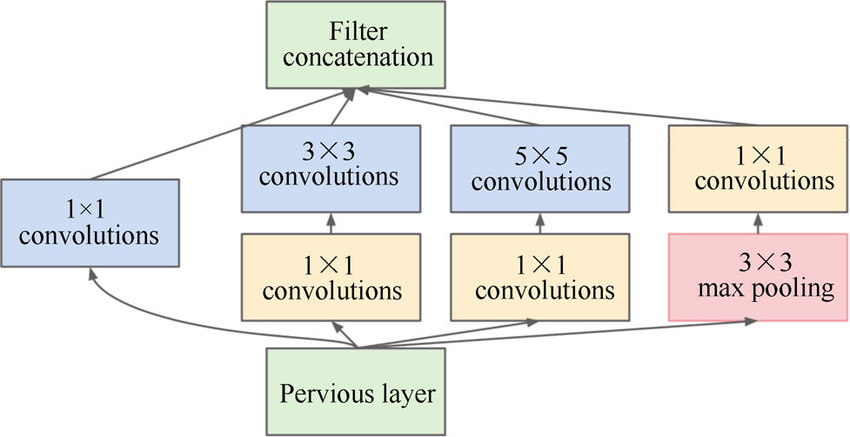
\includegraphics[width=\textwidth]{images/approaches/deep_learning/inception_mod.png}
         \caption{}
         \label{fig:inception}
     \end{subfigure}
     \hfill
     \begin{subfigure}[b]{0.45\textwidth}
         \centering
         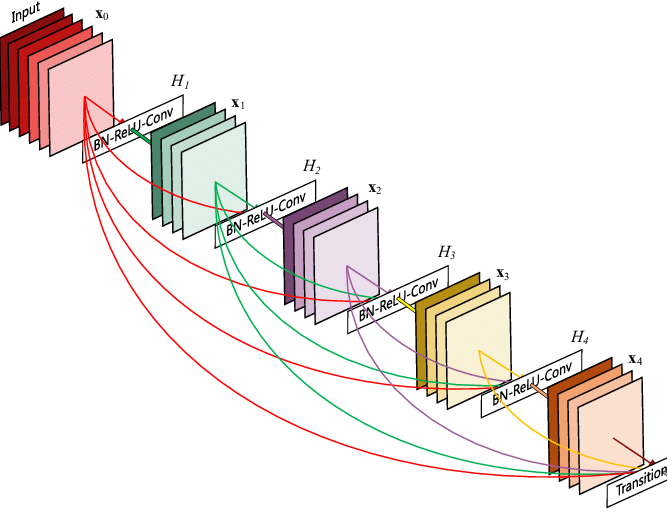
\includegraphics[width=\textwidth]{images/approaches/deep_learning/dense_block.png}
         \caption{}
         \label{fig:dense-block}
     \end{subfigure}
        \caption{(a) Inception module. 1x1 convolutions reduce the dimension along the direction of the number of channels, making the process less computationally expensive.
        Adapted from Szegedy \textit{et al.} 2015~\cite{szegedy2015going}.
        (b) A 5-layer dense block with a growth rate of k = 4.
        Every layer has access to its preceding feature maps, and therefore, to the collective knowledge.
        Each layer adds then new information to this collective knowledge, in concrete k feature maps of information.
        Adapted from Huang \textit{et al.} 2017~\cite{huang2017densely}.}
        \label{fig:inception-dense}
\end{figure}


